% pyFormex manual (we use the python manual class)
%
\documentclass[a4paper]{manual}
%
%% Dirty hack to make Python classes work together with hyperref
\let\pyurl\url
\let\url\relax
%%
\usepackage{hyperref}
%\usepackage[latex2html]{hyperref}
%\usepackage[latex2html,pdftex]{hyperref}
\usepackage{html}
\usepackage{xspace}
\usepackage{graphicx}
\usepackage{subfigure}
%\usepackage[pdftex]{graphicx}
\title{pyFormex manual}
\author{Tim Neels and Benedict Verhegghe}
\release{0.3}
\setshortversion{0.3}
\newcommand{\pyformex}{pyFormex\xspace}
\newcommand{\websiteURL}{http://pyformex.berlios.de\xspace}
%\newenvironment{mycode}{\par\small\sffamily}{} % This should be changed


\begin{document}
\maketitle
\chapter{Introduction}
\label{cha:introduction}

\section{What is \pyformex?}
\label{sec:what-pyformex}
You probably expect to find here a short definition of what \pyformex is and what it can do for you. I may have to disappoint you: describing the essence of \pyformex in a few lines is not an easy task to do, because the program can be (and is being) used for very different tasks. So I will give you two answers here: a short one and a long one.

The short answer is that \pyformex is a program to \emph{generate large structured sets of coordinates by means of subsequent mathematical transformations gathered in a script.}
If you find this definition too dull, incomprehensible or just not descriptive enough, read on through this section and look at some of the examples in this manual and on the \htmladdnormallinkfoot{\pyformex website}{\websiteURL}. You will then probably have a better idea of what \pyformex{} is. 

The initial intention of \pyformex (and probably still its main use) was the rapid design of three-dimensional wireframe structures with a configuration that can easier be obtained through mathematical description than through interactive generation of its sub parts and assemblage thereof.

The example of the stent\footnote{A stent is a tube-shaped structure that is e.g. used to reopen (and keep open) obstructed blood vessels.} in the figure below illustrates this clearly. 

\begin{figure}[h]
  \centering
  \begin{makeimage}
  \end{makeimage}
  \begin{latexonly}
    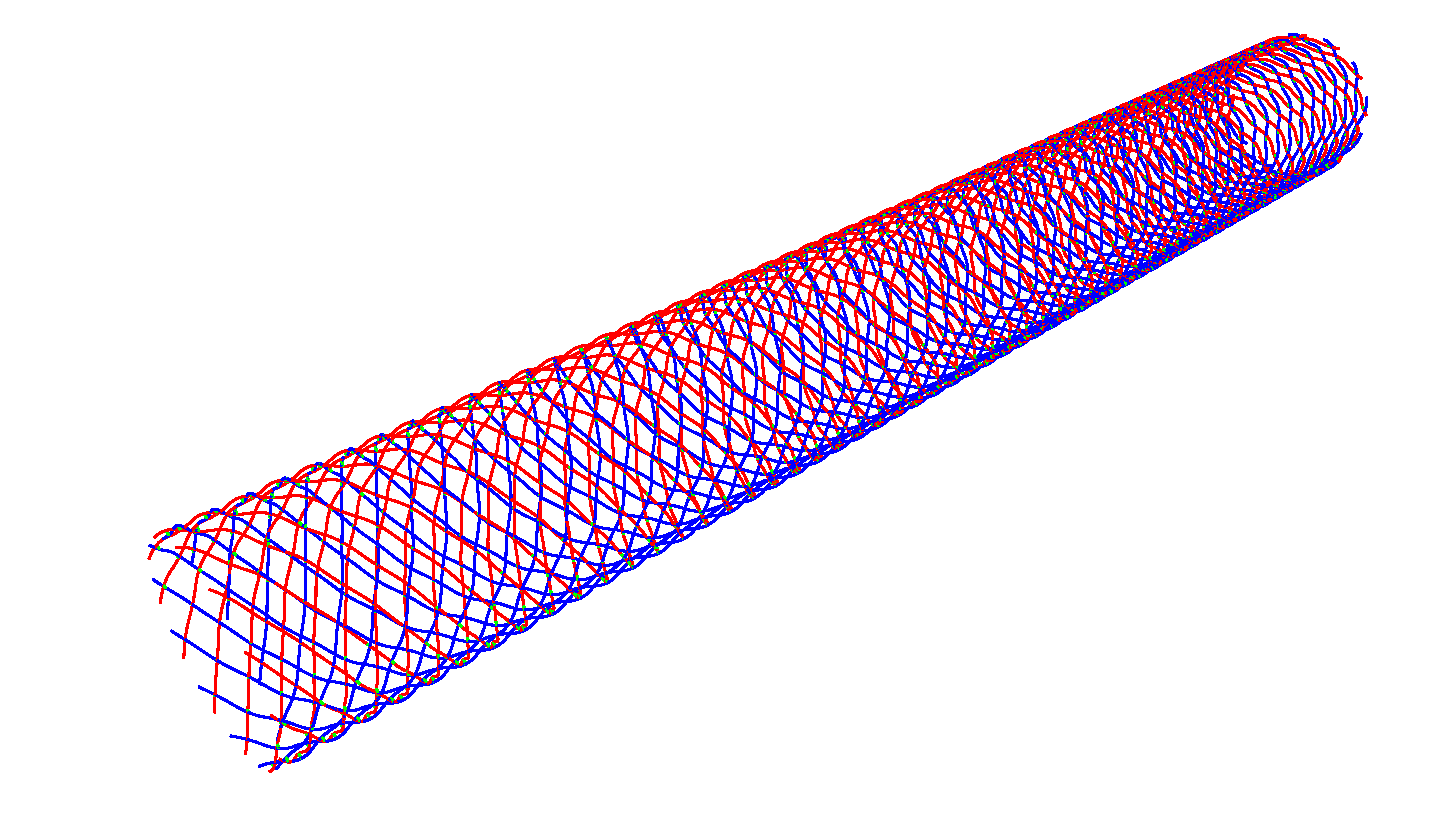
\includegraphics[width=12cm]{images/wirestent}
  \end{latexonly}
  \begin{htmlonly}
    \htmladdimg{../images/wirestent.png}
  \end{htmlonly}  
  \caption{WireStent example.}
\end{figure}


The structure has ...


\section{History}
\label{sec:history}

\section{Quick tutorial for the \pyformex{} GUI}
\label{sec:gui-tutorial}
In the current version () the GUI mainly serves the following purposes:
\begin{itemize}
\item Display a structure in 3D. This includes changing the viewpoint, orientation and viewing distance. Thus you can interactively rotate, translate, zoom.
\item Save a view in one of the supported image formats. Most of the images in this manual and on the \pyformex{} website were created that way. 
\item Changing \pyformex settings (though there aren't many yet that can be changed through the GUI).
\item Running \pyformex scripts, possibly starting other programs and display their results.
\end{itemize}

The GUI does not (yet) provide a means to interactively design a structure, select parts of a structure or set/show information about (parts of) the structure. Designing a structure is done by writing a small script with the mathematical expressions needed to generate it. Any text editor will be suitable for this purpose. The author uses XEmacs, but this is just a personal preference. 
A Python aware editor is preferable though, because that is the language used in \pyformex scripts.
A \pyformex editor integrated into the GUI remains on our TODO list, but it certainly has not our top priority, because general purpose editors are adequate for most of our purposes. 

The best way to learn to use \pyformex is by studying and changing some of the examples. I suggest that you first take a look at the examples included in the \pyformex GUI and select those that display structures that look interesting to you. Then you can study the source code of those examples and see how the structures got built. 
When starting up, \pyformex reads through the Examples directory (this is normally the 'examples' subdirecty located under the pyformex installation dir).  
\menuselection{Examples \sub WireStent}


\section{Quick NumPy tutorial}
\label{sec:numpy-tutorial}
This could be part of the tutorial in chapter 2

%%%%%%%%%%%%%%%%%%%%%%%%%%%%%%%%%%%%%%%%%%%%%%%%%%%%%%%%%%%%%%%%%%%%%%%%%%%
\chapter{\pyformex --- a tutorial}
{\label{cha:tutorial}


%%
\section{Introduction}
\label{sec:intro-tut}
\pyformex is a Python implementation of Formex algebra. Using \pyformex, it is very easy to  generate large geometrical models of 3D structures by a sequence of mathematical transformations. It is especially suited for the automated design of spatial frame structures. But it can also be used for other tasks, like finite element preprocessing, or just for creating some nice pictures.

By writing a very simple script, a large geometry can be created by copying, translating, rotating,... Formices. \pyformex will interpret this script and draw what you have created. This is clearly very different than the traditional way of creating a model, like CAD. There are two huge advantages about using \pyformex

\begin{itemize}
\item It is especially suited for the automated design of spatial frame structures. A dome, arc, hypar,... can be rather difficult to draw with CAD, but when using mathematical transformations, it becomes a piece of cake!
\item Using a script makes it very easy to apply changes in the geometry: you simply modify the script and let \pyformex play it again. For instance, you can easily change an angle, the radius of a dome, the ratio f/l of an arc,... Using CAD, you would have to make an entirely new drawing! This is also illustrated in fig \ref{scallops}: these domes where all created with the same script, but with other values of the parameters.
\end{itemize}

\begin{figure}[tbp,h]
  \centering
  \begin{makeimage}
  \end{makeimage}
  \begin{latexonly}
    \subfigure[A basic Scallopdome]{\label{scallop}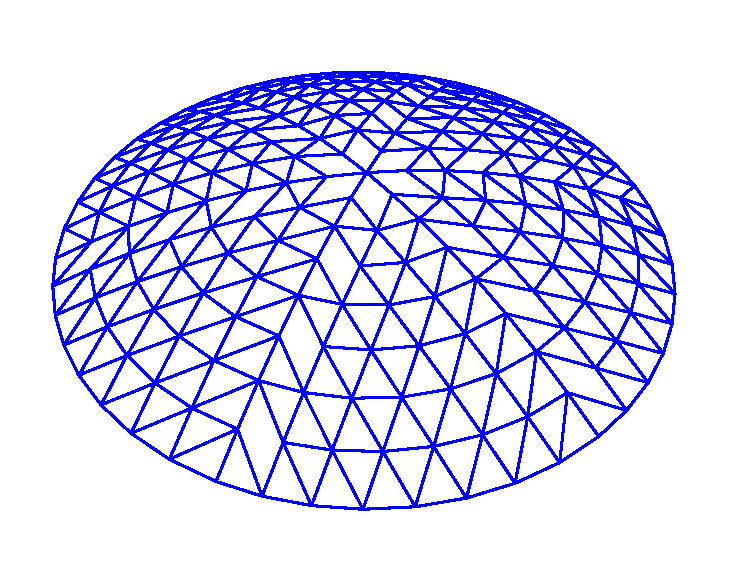
\includegraphics[width=5cm]{images/scallopdome-000}}
    \hfill
    \subfigure[Another Scallopdome]{\label{scallop2}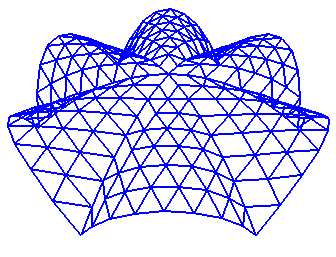
\includegraphics[width=5cm]{images/scallopdome-001}}
    \hfill
    \subfigure[Yet another Scallopdome]{\label{scallop3}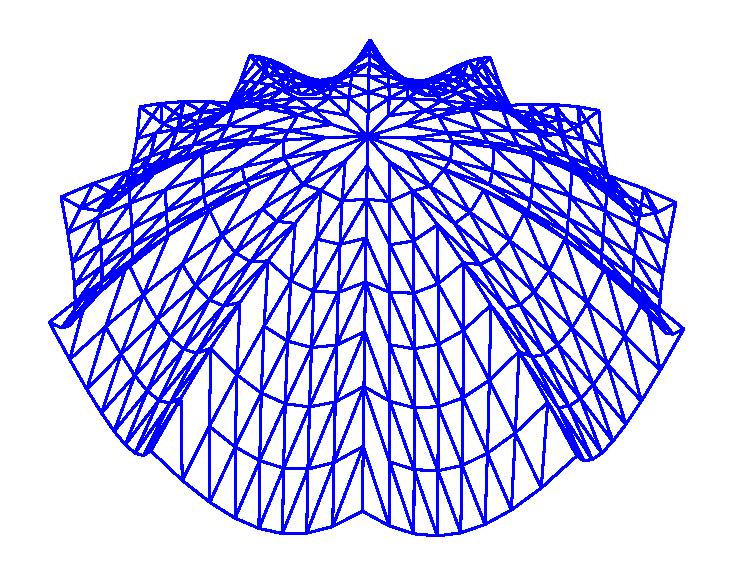
\includegraphics[width=5cm]{images/scallopdome-002}}
  \end{latexonly}
  \begin{htmlonly}
%    \htmladdimg[WIDTH="300"]{../images/scallopdome-000.png}
    \htmladdimg{../images/scallopdome-000.png}
    \htmladdimg{../images/scallopdome-001.png}
    \htmladdimg{../images/scallopdome-002.png}
  \end{htmlonly}
  \caption{Same script, different domes} \label{scallops}
\end{figure}

As mentioned, \pyformex is based on the programming language Python \footnote{\url{http://www.python.org}}. This implies that the scripts are also Python-based. It's a very easy language, but if you're interested in reading more, there is a very good tutorial available on \url{http://docs.python.org/tut/}. However, if you're only using Python to write \pyformex-scripts, the tutorial you're reading right now should be enough. 


%%
\section{Getting started}
\label{sec:getting-started}
This section holds some basic information on how to use Python and \pyformex. 

\begin{itemize}
\item To open \pyformex, double click on the file \file{pyformex} in the installation directory, or type \emph{pyformex} in the terminal. Using the terminal can be very useful, because errors that are created while running the script will appear in the terminal. This can provide you with useful information when something goes wrong with your script.
\item To create a new \pyformex-script, just open a new file with your favorite text-editor and save it as \file{myproject.py}.
\item To edit a script, you can
	\begin{itemize}
	\item Open it with your favorite text-editor
	\item Select 'open' from the 'file'-menu and browse to your script. At this point, the script will be loaded but nothing will 		happen. Now you can select 'edit' from the 'file'-menu, and the script will open in the default text-editor. This default editor 		can be changed in the file \file{.pyformexrc} in the installation directory.
	This way of editing your script makes it possible to immediately draw changes you applied in the script (without reopening 		the file).  Just select 'play' from the 'file'-menu.
	\end{itemize}
\item To play a script, you can
	\begin{itemize}
	\item Select 'open' from the 'file'-menu and browse to your script. Then select 'play' from the 'file'-menu.
	\item Type \emph{pyformex myproject.py} in the terminal. This will open \pyformex and play your script at the same time.
	\item To play a script without using the GUI (for example in finite element preprocessing, if you only want to write an 		output file, without drawing the structure), type \emph{pyformex --nogui myproject.py}
	\end{itemize}
\item When writing a script in Python, there are some things you should keep in mind:
	\begin{itemize}
	\item When using a function that requires arguments, an argument list must have any positional arguments followed by any keyword arguments, where the keywords must be chosen from the formal parameter names. It's not important whether a formal parameter has a default value or not. No argument may receive a value more than once -- formal parameter names corresponding to positional arguments cannot be used as keywords in the same calls. 
Simply put: you can either set the arguments in the right order and only give their value, or you can give arguments by their name and value. This last option holds some advantages: not only is it easier to check what you did, but sometimes a function has many arguments with default values and you only want to change a few.
If this isn't entirely clear yet, just look at the examples later in this tutorial or check the Python tutorial.
	\item Indentation is essential in Python. Indentation is Python's way of grouping statements. In straight-forward scripts, indentation is not needed (and forbidden!), but when you use an if-statement for example, the body of the statement has to be indented. A small example might make this clear. Also notice the ':' 
\begin{verbatim}
	print 'properties'
	for key, item in properties.iteritems():
	    print key, item
\end{verbatim}
	\item If you want to use functions from a seperate module (like \module{properties}), you add a line on top of the script
\begin{verbatim}
	from properties import *
\end{verbatim}
All functions from that module are now available.
	\item The hash character, "\#", is used to start a comment in Python.
	\item Python is case sensative.
	\end{itemize}
\end{itemize}


%%
\section{Geometric model}
\label{sec:geom}


\subsection{Creating a Formex}
\label{subsec:create}

\subsubsection{What is a Formex}
A Formex is a numarray of order 3 (axes 0,1,2) and type Float.
A scalar element represents a coordinate (F:uniple).

    A row along the axis 2 is a set of coordinates and represents a point
    (node, vertex, F: signet).
    For simplicity's sake, the current implementation only deals with points
    in a 3-dimensional space. This means that the length of axis 2 is always 3.
    The user can create Formices (plural of Formex) in a 2-D space, but
    internally these will be stored with 3 coordinates, by adding a third
    value 0. All operations work with 3-D coordinate sets. However, a method
    exists to extract only a limited set of coordinates from the results,
    permitting to return to a 2-D environment.

    A plane along the axes 2 and 1 is a set of points (F: cantle). This can be
    thought of as a geometrical shape (2 points form a line segment, 3 points
    make a triangle, ...) or as an element in FE terms. But it really is up to
    the user as to how this set of points is to be interpreted.

    Finally, the whole Formex represents a set of such elements.

    Additionally, a Formex may have a property set, which is an 1-D array of
    integers. The length of the array is equal to the length of axis 0 of the
    Formex data (i.e. the number of elements in the Formex). Thus, a single
    integer value may be attributed to each element. It is up to the user to
    define the use of this integer (e.g. it could be an index in a table of
    element property records).
    If a property set is defined, it will be copied together with the Formex
    data whenever copies of the Formex (or parts thereof) are made.
    Properties can be specified at creation time, and they can be set,
    modified or deleted at any time. Of course, the properties that are
    copied in an operation are those that exist at the time of performing
    the operation.   

Simply put: a Formex is a set of elements, and every element can have a property number.

\subsubsection{Creating a Formex using coordinates}
The first and most useful way to create a Formex is by specifying it's nodes and elements in a 3D-list.  

\begin{verbatim}
	F=Formex([[[0,0],[1,0],[1,1],[0,1]]])
\end{verbatim}
%fig?

This would create a Formex F, which has the nodes (0,0), (0,1), (1,1) and (0,1). These nodes are all part of a single element, thus creating a square plane. This element is also the entire Formex.
On the other hand, if you would change the position of the square brackets like in the following example, then you'd create a Formex F which is different from the previous. The nodes are the same, but the connection is different. The nodes (0,0) and (1,0) are linked together by an element, and so are the nodes (1,1) and (0,1). The Formex is now a set of 2 parallel bars, instead of a single square plane. 
\begin{verbatim}
	F=Formex([[[0,0],[1,0]],[[1,1],[0,1]]])
\end{verbatim}
%fig?

If we want to define a Formex, similar to the square plane, but consisting of the 4 edges instead of the actual plane, we have to define four elements and combine them in a Formex.
\begin{verbatim}
	F=Formex([[[0,0],[0,1]], [[0,1],[1,1]], [[1,1],[1,0]], [[1,0],[0,0]]])
\end{verbatim}

The previous examples were limited to a 2-D environment for simplicity. Of course, we could add a third dimension. For instance, it's no problem defining a pyramid consisting of 8 elements ('bars').
\begin{verbatim}
	F=Formex([[[0,0,0],[0,1,0]], [[0,1,0],[1,1,0]], [[1,1,0],[1,0,0]], [[1,0,0],[0,0,0]], [[0,0,0],[0,1,0]], [[0,0,0],[0.5,0.5,1]], 		[[1,0,0],[0.5,0.5,1]], [[1,1,0],[0.5,0.5,1]], [[0,1,0],[0.5,0.5,1]]])
\end{verbatim}
%fig
However, as you can see, even in this very small example the number of nodes, elements and coordinates you have to declare becomes rather large. Defining large Formices using this method would not be practical. This problem is easily overcome by copying, translating, rotating,... a smaller Formex - as will be explained in the rest of this chapter - or by using patterns.
 
\subsubsection{Creating a Formex using patterns}

The second way of creating a new Formex, is by defining patterns. In this case, a line segment pattern is created from a string.

%remove this part?
    This function creates a list of line segments where all nodes lie on the
    grid points of a regular grid with unit step.
    The first point of the list is [0,0]. Each character from the given
    string is interpreted as a code specifying how to move to the next node.
    Currently defined are the following codes:
    0 = go to origin [0,0]
    1 = East, 2 = North, 3 = West, 4 = South, 5 = NE, 6 = NW, 7 = SW, 8 = SE
    / = go to the next point without connecting.
    The resulting list is directly suited to initialize a Formex in the
    (x,y)-plane.
%until here

This method has important restrictions, since it can only created lines, in a 3-D environment, on a regular grid. However, it can be a much easier and shorter way to define a simple Formex. This is illustrated by the difference in length between code 3 and code ref 4, although they define the same Formex.%ref aanpassen
\begin{verbatim}
	F=Formex(pattern('1234'))
\end{verbatim}

Some simple patterns are defined in \module{simple.py} and are ready for use. These patterns are stacked in a dictionary called 'Patterns'. Items of this dictionary can be accessed like \code{Patterns['cube']}.
\begin{verbatim}
	from simple import *
	c=Formex(pattern(Pattern['cube']))
	draw(c)
\end{verbatim}

\subsubsection{Creating a Formex using coordinates from a file}
In some cases, you might want to read coordinates from a file an combine them into a Formex. This is possible with the module \module{file2formex} and it's function \function{fileFormex()}. Each point is connected to the following, forming an element (bar).
The next file ('square.txt') would create the same Formex as the previous example. %ref?
\begin{verbatim}
	0,0,0
	0,1,0
	1,1,0
	1,0,0
\end{verbatim}
\begin{verbatim}
	from file2formex import *
	F=fileFormex('square.text', closed='yes')
\end{verbatim}

\subsection{Adding property numbers}
\label{subsec:propnr}
Each Formex element can have a property number. Each property number is represented by another color when the Formex is drawn. This is the first reason why you could use property numbers: to make your drawing more transparent or just more beautiful. However, these numbers can also be used as an entry in a dictionary of properties - thus linking the element with a property. This property can be about anything, but in finite element processing this would be the element section, material, loads,... The use of properties in this way will be futher explained in \ref{sec:props}.
Property numbers can be specified at creation time, and they can be set, modified or deleted at any time.  
\begin{verbatim}
>>> F=Formex(pattern('1234'),[5])
>>> print F.prop()
>>> G=Formex(pattern('1234'),[6,8,2,4])
>>> print G.prop()
>>> F.setProp([6,7])
>>> print F.prop()
>>> G.setProp([6,7,8,9])
>>> print G.prop()

[5 5 5 5]
[6 8 2 4]
[6 7 6 7]
[6 7 8 9]
\end{verbatim}

\subsection{Drawing a Formex}
\label{subsec:drawing}
Of course, you'd want to see what you have created. This is accomplished by the \function{draw()} function. 
\begin{verbatim}
	F=Formex([[[0,0,0],[0,1,0]], [[0,1,0],[1,1,0]], [[1,1,0],[1,0,0]], [[1,0,0],[0,0,0]], [[0,0,0],[0,1,0]], [[0,0,0],[0.5,0.5,1]], 		[[1,0,0],[0.5,0.5,1]], [[1,1,0],[0.5,0.5,1]], [[0,1,0],[0.5,0.5,1]]])
	draw(F)
\end{verbatim}

It also possible to draw multiple Formices at the same time.
\begin{verbatim}
	F=Formex([[[0,0,0],[0,1,0]], [[0,1,0],[1,1,0]], [[1,1,0],[1,0,0]], [[1,0,0],[0,0,0]], [[0,0,0],[0,1,0]], [[0,0,0],[0.5,0.5,1]], 		[[1,0,0],[0.5,0.5,1]], [[1,1,0],[0.5,0.5,1]], [[0,1,0],[0.5,0.5,1]]])	
	G=Formex(pattern('1234'))
	draw(F+G)
\end{verbatim}
 
It might be important to realize that even if you don't draw a particular Formex, that doesn't mean you didn't create it!

Now, when you are creating a large geometry, you might be interested in seeing the different steps in the creation. To remove all previously drawn Formices, you can use \function{clear()}  what sweepes the screen clean. If you want to see a certain step in the creation longer than the default time, use \function{sleep(t)}, with 't' the delay (in seconds) before executing the next command.
\begin{verbatim}
	F=Formex(pattern('164'))
	draw(F)
	G=F.replic(5,1,0)
	clear()
	draw(G)
\end{verbatim}


\subsection{Information about a Formex}
\label{subsec:info}
There are a number of functions available that return information about a Formex. Especially when using \pyformex as finit element preprocessor, the most useful functions are:
%tabel?
\begin{table}[h]
	\begin{tabular}{*{5}{rl}}
F.nelems()				& Return the number of elements in the formex\\
F.nnodes() 			& Return the number of nodes in the formex.\\
F.prop() 				& Return the properties as a numpy array.\\
F.bbox()				& Return the bounding box of the Formex.\\
F.center()				& Return the center of the Formex.\\
F.nodesAndElements() 	& Return a tuple of nodal coordinates and element connectivity.\\
	\end {tabular}
\end{table}

\function{nodesAndElements} is very important in finite element processing. It returns all nodes and all elements of the Formex in a format useful for FE processing. A tuple of two arrays is returned. The first is float array with the coordinates of the unique nodes of the Formex. The second is an integer array with the node numbers connected by each element.
\begin{verbatim}
>>> from simple import *

>>> c = Formex(pattern(Pattern['cube']))
>>> draw(c)
>>> nodes,elems = c.nodesAndElements()
>>> print 'Nodes'
>>> print nodes
>>> print 'Elements'
>>> print elems

Nodes
[[ 0.  0. -1.]
 [ 1.  0. -1.]
 [ 0.  1. -1.]
 [ 1.  1. -1.]
 [ 0.  0.  0.]
 [ 1.  0.  0.]
 [ 0.  1.  0.]
 [ 1.  1.  0.]]
Elements
[[4 5]
 [5 7]
 [7 6]
 [6 4]
 [4 0]
 [5 1]
 [7 3]
 [6 2]
 [0 1]
 [1 3]
 [3 2]
 [2 0]]
\end{verbatim}

\subsection{Changing the Formex}
\label{subsec:changing}

%\subsection{Create copies, concatenations,subtractions}\label{copy F}

%\subsection{Affine transformations}

%\subsection{Non-affine transformations}

%\subsection{Transformations that change the topology}


%
\section{Adding properties}
\label{sec:props}


%
\section{Export to finite-elements program}


%
\section{Tips and Tricks}

Some of these tips are already mentioned in the previous sections, but......
\begin{itemize}
\item Starting \pyformex using the terminal can be very useful. Errors that are created while running the script will appear in the terminal, you can use the 'print'-function to check a result,... This can be a very useful when controlling your script
\item nog wat hints 
\end{itemize}





%%%%%%%%%%%%%%%%%%%%%%%%%%%%%%%%%%%%%%%%%%%%%%%%%%%%%%%%%%%%%%%%%%%%%%%%%%%
\chapter{\pyformex --- reference manual}
{\label{cha:reference}

\section{formex --- the base module}
{\label{sec:formex}

This module contains all the basic functionality for creating, structuring and transforming sets of coordinates.

\begin{classdesc}  {Formex}{data=[[[]]],prop=None}
A class to hold a structured set of coordinates. A \class{Formex} is a three dimensional array of float values. The array has a shape \code{(nelems,nnodel,3)}. Each slice \code{[i,j]} of the array contains the three coordinates of a point in space. We will also call this a \emph{node}. Each slice \code{[i]} of the array contains a connected set of nnodel points: we will refer to it as an \emph{element}. 

It is up to the user on how to interprete this connection: two connected nodes will usually represent a line segment between these two points. An element with three nodes however could just as well be interpreted as a triangle or as a (possibly curved) line. And if it is a triangle, it could be either the circumference of the triangle or the part of the plane inside that circumference. As far as the Formex class concerns, each element is just a set of points. 

All elements in a \class{Formex} must have the same number of points, but you can construct \class{Formex} instances with any (positive) number of nodes per element. When \code{nnodel==1}, the \class{Formex} contains only unconnected nodes (each element is just one point).

One way of attaching other data to the \class{Formex}, is by the use of the 'property' attribute. The property is an array holding one integer value for each of the elements of the Formex. The use of this property value is completely defined by the user. It could be a code for the type of element, or for the color to draw this element with. Most often it will be used as an index into some other (possibly complex) data structure holding all the characteristics of that element. 

By including this property index into the Formex class, we make sure that when new elements are constructed from existing ones, the element properties are automatically propagated.

\end{classdesc}

\begin{memberdesc}  [array]{f}
A three dimensional array of float values. The array has a shape (nelems,nnodel,3). Each slice [i,j] of the array contains the three coordinates of a point in space. We will also call this a \emph{node}. Each slice [i] of the array contains a connected set of nnodel points: we will refer to it as an \emph{element}. It is up to the user on how to interprete this connection: two connected nodes will usually represent a line segment between these two points. An element with three nodes however could just as well be interpreted as a triangle or as a (possibly curved) line. And if it is a triangle, it could be either the circumference of the triangle or the part of the plane inside that circumference.   
\end{memberdesc}



\end{document}
